% !TEX root = ../thesis-example.tex
%
\chapter{Introduction}
\label{ch:introduction}
%
%\cleanchapterquote{L'instrument est un compromis instable\\entre des qualités non-convergentes.}{Bernard Sève}{(L'instrument de musique: une étude philosophique \cite{seve_instrument_2013})}

\cleanchapterquote{MUSIQUE. \textit{Petit orchestre en train de s'accorder doucement.}\\
PAROLES. —~Pitié! (\textit{Orchestre. Plus fort.}) Pitié! (\textit{L'orchestre faiblit, se tait.}) Combien de temps encore à moisir ici dans le noir ? (Avec dégoût.) Avec toi! (\textit{Un temps.})}
{Samuel Beckett}{\textit{paroles et musique}. Pièce radiophonique. 1962.}

%\cleanchapterquote{—~Dis papa, ça veut dire quoi FM sur ma radio ?\\
%					Formation Musicale ?\\
%					—~mmm... peut-être oui.}
%{Olga Goudard}{questions diverses. 2019.}


\vspace*{\fill}

%\Pierre{ l'introduction doit présenter le titre : représentation, contrôle, desgin interactif, instrument de musique et instrument de musique numérique (pas forçément dans cet ordre)}

%\Pierre{ je pense que tu devrais ici repartir du début : tes motivations pour ce sujet et quels sont les notions que tu dois absolument présenter pour que l'on comprenne ta problématique. Typiquement, une intro de thèse = contexte -> problématique/hypothèses -> annonce du plan}
\noindent {\Large \textbf{Rewind~/~Record~/~Fast-Forward}}

\noindent J'ai commencé l'étude d'un ``vrai'' instrument de musique --~le saxophone~-- en école de musique à l'âge de 12 ans, mais n'ai réalisé que des années plus tard que le premier instrument de musique que j'avais pratiqué avait six touches et deux contrôleurs continus: REC, PLAY, PAUSE, STOP, RWD, FWD, un contrôle de volume et un sélecteur de fréquence radio. Né au moment de la commercialisation du Walkman™ et de la ``libération des ondes'', j'ai rapidement eu entre les mains cet objet que peu auraient appelé ``instrument de musique'' à cette époque (sauf dans certains lieux qui m'étaient encore inconnus à cet âge), qui permettaient pourtant de jouer des sons, des sons venant d'ailleurs ou des sons personnels, enregistrés ``à la main''. Le balladeur, comme son nom l'indique, permettait d'emmener sa musique partout (à la condition d'avoir des piles chargées), chez soi comme à l'extérieur, de se plonger comme par magie dans des paysages sonores au beau mileu de la forêt ou de la ville, et particulièrement durant les ``déplacements'', trajets de bus ou de voiture dont il fournissait la bande-son. L'écoute au walkman a probablement constitué la pratique musicale principale de toute ma génération en nombres d'heures passées sur son instrument.
\begin{wrapfigure}[4]{r}{0.25\textwidth}
	\vspace{-6.2em}
	\captionsetup{format=plain}
	\centering
 	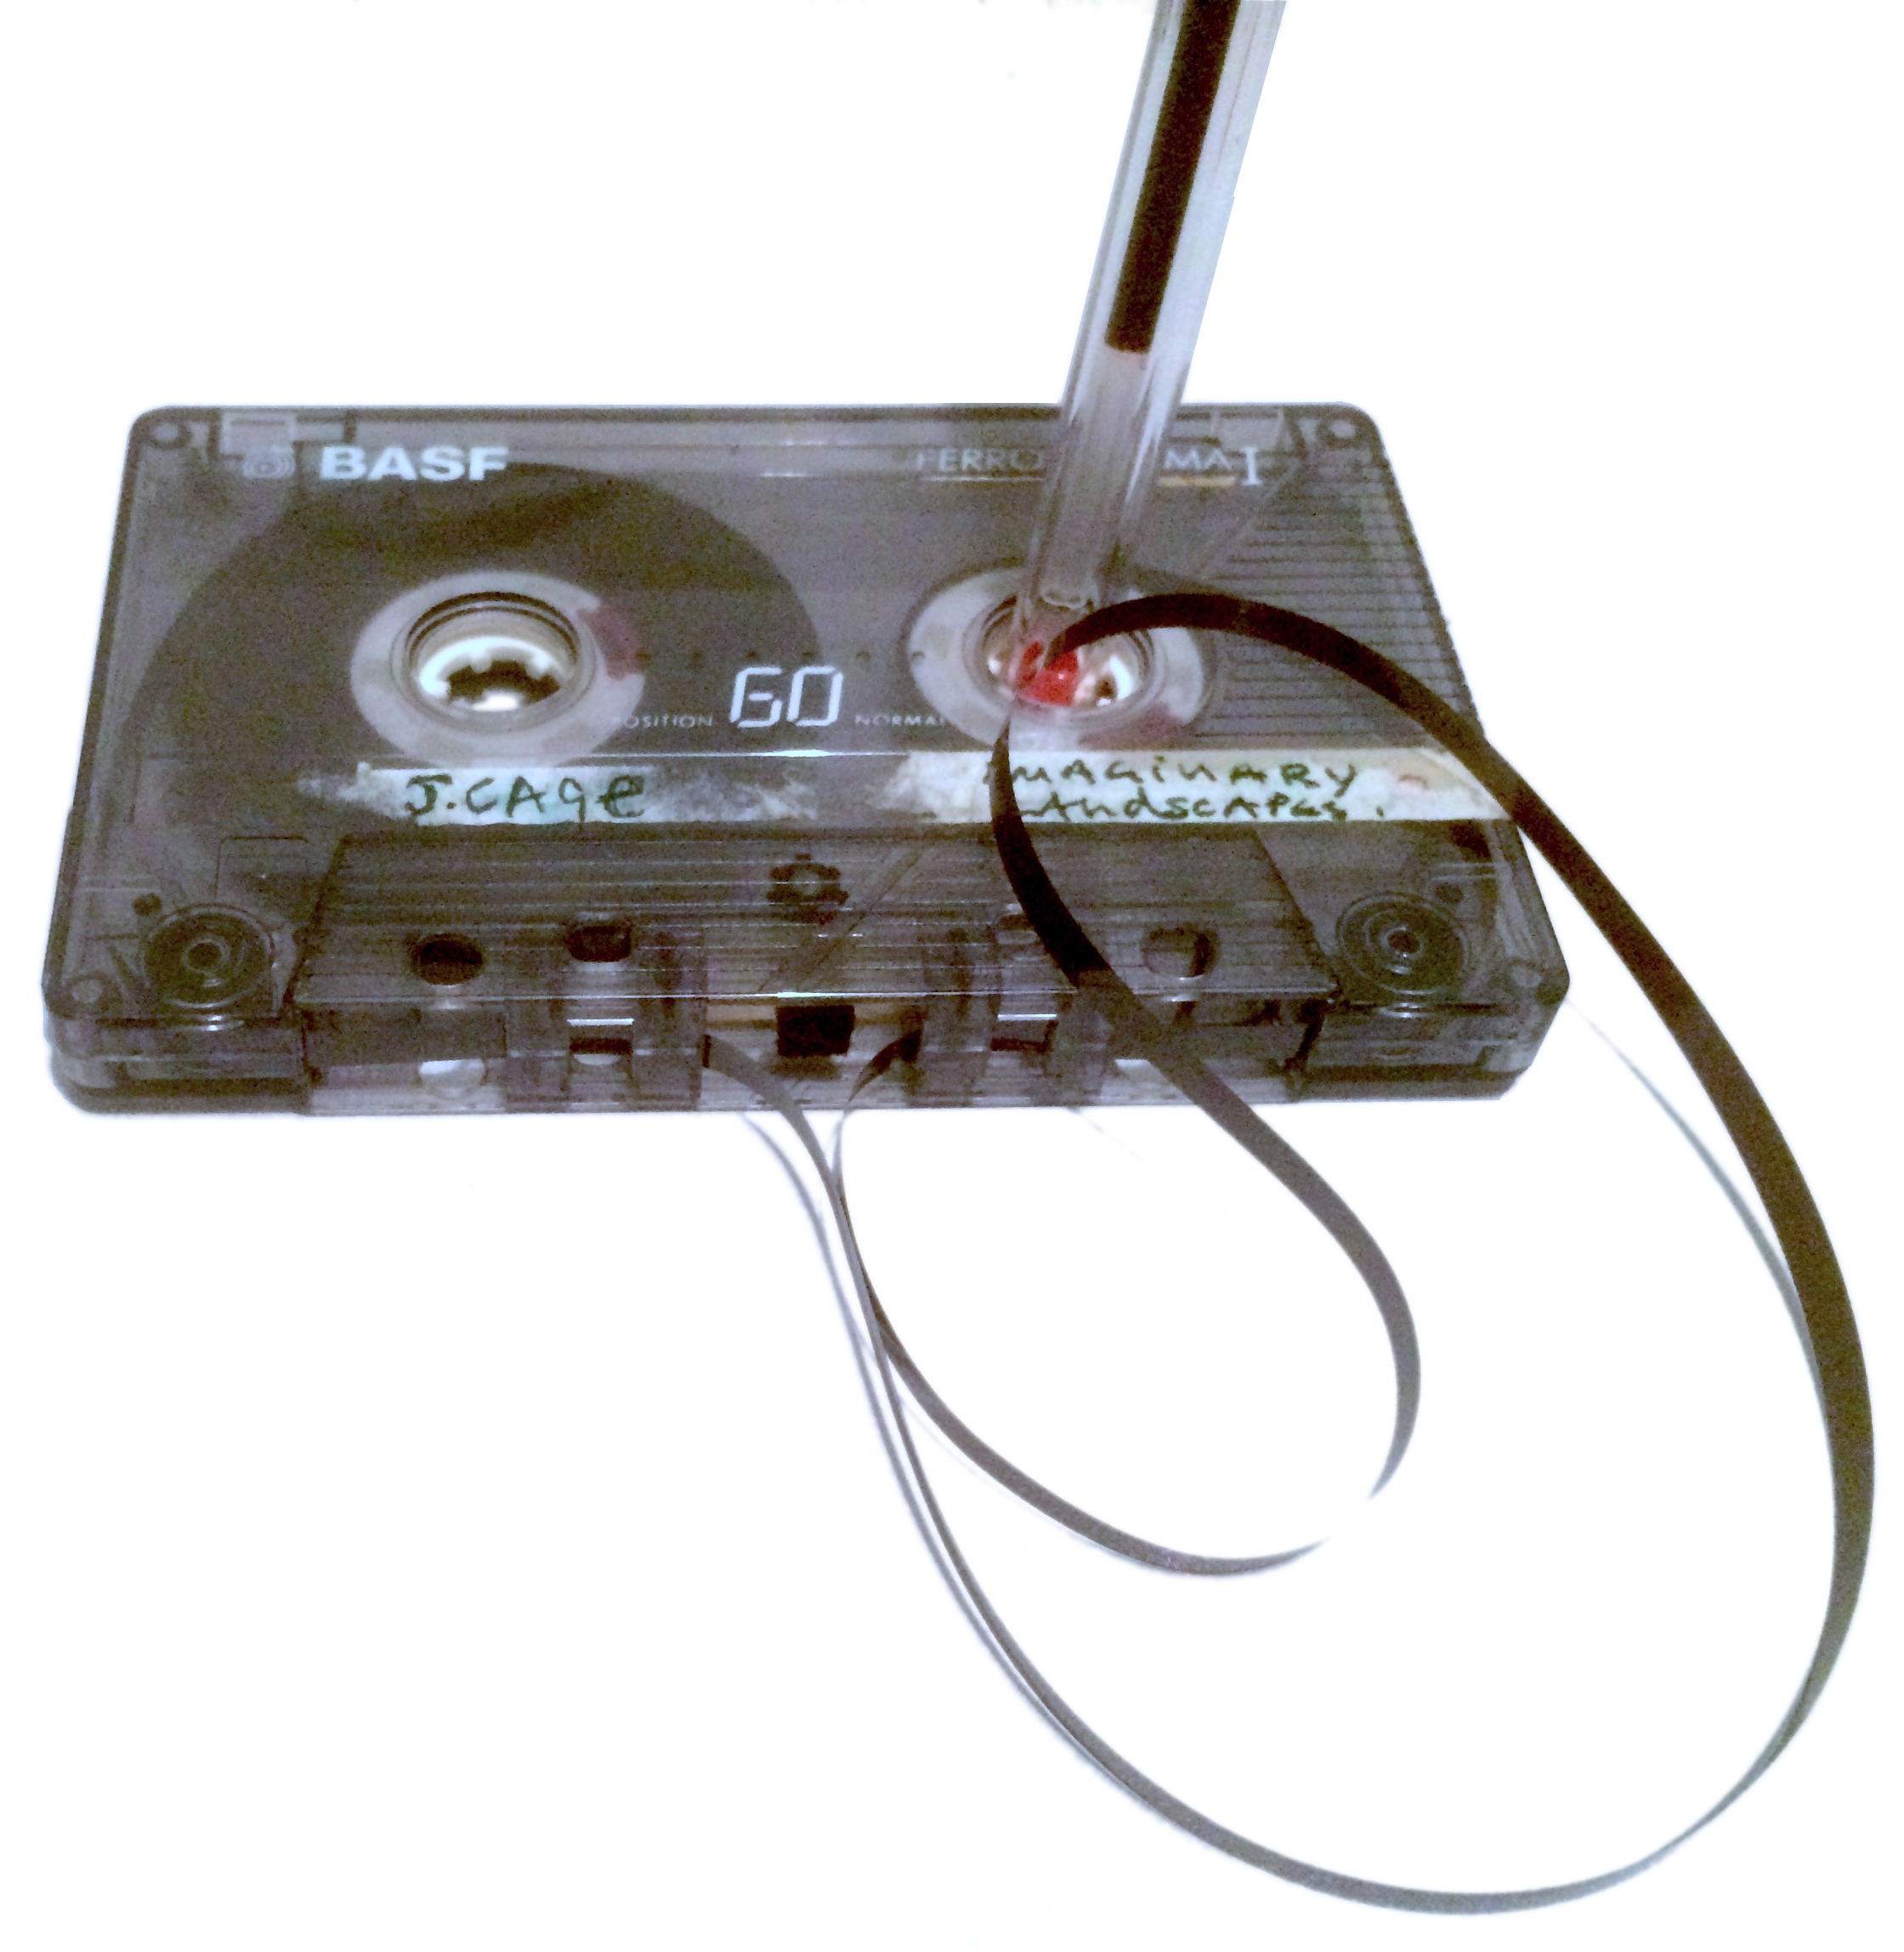
\includegraphics[width=0.56\textwidth]{gfx/01_preamble/K7.png}
 	%\vspace{-2em}
	%\caption[Walkman.]{Walkman.}
 	\label{fig:preamble:walkman}
\end{wrapfigure}
\par
%\indent Aurais-je été en droit d'appeler mon balladeur-enregistreur un ``instrument'' ? Il existait bien un répertoire pour cet instrument, virtuellement \textit{tout} le répertoire en fait, à portée de main dans les médiathèques et chez les disquaires, mais aucun professeur enseignant sa pratique et en premier lieu, aucun musicien jouant d'un tel instrument en concert. Pourtant il y avait un public et je n'étais pas le seul auditeur; l'échange entre amis de compilations sur cassettes audio nous permettait de partager des morceaux, et à défaut d'en être les auteurs, nous étions les auteurs de nos sélections musicales.\\
\indent Une dizaine d'années plus tard, la dédicace de Pierre Schaeffer à son père que je découvre à l'ouverture de l'imposant \textit{Traité des objets musicaux} fait écho à cette question : \iquote{À la mémoire de mon père, violoniste, dont je transmets le précepte : Travaille ton instrument}. 
Ce précepte qui prend la forme d'une injonction laisse imaginer la scène du père qui ordonne au petit Pierre d'aller faire ses gammes. Mais quel est donc l'instrument que Pierre Schaeffer semble avoir suffisamment travaillé pour reprendre à son compte ce précepte en ouverture de son ouvrage majeur ? Le disque à sillon fermé ? Le \textit{Phonogène} ? Le son lui-même ? Où s'agirait-il davantage de sa propre perception auditive, dont il entreprend l'étude systématique pour en déchiffrer les ``modes d'écoute'' comme on parle de ``mode de jeu'' ?\\
\indent Le présent travail de recherche a commencé après plus de 15 années passées à concevoir, fabriquer, programmer, pratiquer et écouter des instruments de musique à l'aide d'ordinateurs. J'ai créé durant ces années diverses sortes d'applications, d'instruments, d'installations, d'outils, dans différents contextes : spectacle vivant, installations multimédia, ateliers pédagogiques, expositions muséographiques, émissions de radio, projets de recherche, etc. Il est sûrement vain de vouloir discriminer parmi tous ces objets lesquels constituent des instruments de musique et lesquels n'en sont pas, mais il me semble intéressant de constater que ces développements posent à chaque fois, sous différents angles, la question du rapport de musicalité avec la machine. C'est ce constat qui m'a amené à réfléchir sur ma pratique et sur la notion d'\gls{DMI}\footnote{Les acronymes utilisés dans cette thèse sont définis dans le glossaire et clickables (dans la version numérique de ce document!) pour y accéder directement.} pour essayer d'en cerner les contours, ou du moins, d'en percevoir les lignes de fuite.\\
\indent Poser la question de sa représentation, quand le medium numérique fait voler l’objet en éclat ainsi que les traditions musicales qu’il sous-tend, pose imanquablement celle des motivations pour lesquelles nous construisons des instruments, et par suite, des raisons pour lesquelles nous inventons, pratiquons, écoutons la musique. De cela découlent les multiples manières dont nous jouons avec le réel, avec les objets, avec les sons pour produire cet étrange --~et pourtant si familière~-- vibration de l'air.\\
\indent La notion de \gls{DMI} embrasse ces problématiques, complexes sur le plan technique, mais davantage encore sur le plan sociologique, esthétique et philosophique. La façon dont nous créons la musique et la manière dont nous l’écoutons a tellement changé en un siècle qu’il semble désuet de tenter de l’aborder sur un plan purement technique, tant celle-ci semble promise à bouleverser encore davantage nos usages dans l’avenir. Le travail présenté dans cette thèse ne prétend pas répondre à ces vastes questions mais tâchera, autant que possible, de ne pas perdre de vue les raisons profondes du désir musical, pour en expliciter les conséquences sur certains choix de design -- perspective nécessaire qui s'inscrit, de toute évidence, dans le travail de mon instrument.

\section{Une thèse transdisciplinaire}

\noindent Cette thèse a été l'objet d'un contrat doctoral soutenu par le Collegium Musicæ\footnote{Le \textit{Collegium Musicæ} de Sorbonne Université est un institut qui rassemble musiciens, chercheurs et enseignants-chercheurs autour de la création, la recherche, la conservation et la pratique musicale. Il rassemble dix organismes de recherche et de formation spécialisés dans le domaine musical. Site \url{http://www.collegium.musicae.sorbonne-universite.fr}}, dont la mission est de promouvoir l'interdisciplinarité entre différents acteurs institutionnels œuvrant dans le champ de la musique et de la recherche. En l'occurence, cette thèse a été co-dirigée par Pierre Couprie, musicologue à l'\gls{IReMus} et Jean-Dominique Polack et Hugues Genevois, chercheurs de l'équipe \gls{LAM}. En se situant entre les domaines distincts des sciences et de l'ingénierie d'une part et de la musicologie d'autre part, cette thèse est la tentative d'une étude des \glspl{DMI} prenant ces deux dimensions en compte.\\
\indent Par ailleurs, ce travail de recherche théorique est soutenu par des développements techniques disponibles librement sur Internet et dont j'espère qu'ils pourront profiter à la communauté des musiciens intéressés par ces outils.\\
\indent Enfin, elle s'appuie sur des performances musicale mettant en œuvre ces développements pour confronter la théorie à la pratique tout autant que pour affiner la théorie sur la base de l'observation de ces pratiques. Elle constitue donc un travail de une recherche à la fois basée sur la pratique et dirigée par la pratique.\\
\indent Cette transdisciplinarité propre à la musique, qui convoque les sciences acoustiques, cognitives, informatiques, l'ingénierie de l'instrument, l'histoire de son évolution, (...) a donné lieu à l'émergence de communautés illustrant l'échange nécessaire entre les disciplines pour tenter de comprendre la manière dont elle se construit et se manifeste dans des pratiques situées aux esthétiques multiples. Le Collegium Musicæ en est un parfait exemple, ainsi que le sont les conférences sur les nouvelles lutheries --~notamment numériques~-- telles les \gls{JIM}, \gls{NIME} ou \gls{ICLI} qui rassemblent chercheurs en sciences exactes et humaines, musiciens, luthiers, pédagogues et compositeurs présentant leurs réflexions, leurs pratiques, leurs œuvres, leurs instruments, leur outils dans le but de partager les points de vue autour de ces questions.


\section{Qu'entend-on par ...}

\noindent Il s'agit ici de donner quelques éléments permettant de préciser la signification donnée à un certain nombre de termes dans ce document.

\subsection*{``Représentation...}

\noindent Le terme ``représentation'' recouvre un très vaste champ sémantique. Si son étymologie évoque le fait de ``rendre de nouveau présent'', la représentation passe aussi par l'image --~réelle ou mentale~--, distincte de l'original représenté, que l'on se fait de quelque chose. La question de la représentation (ou plutôt, des représentations) dans les lutheries numériques est envisagée sous différents angles, et présente ainsi des significations variables dans ce document : 
\vspace{-1em}
\begin{itemize}[noitemsep]
\item la représentation organologique des \glspl{DMI}, en particulier les manières variées dont il se présente comme agencements modulaires (ch. \ref{ch:ephemeral}) en contraste avec les représentations plus monolithiques de l'instrument classique;
\item la représentation de ce que l'on appelle communément ``le geste musical'' du point de vue des \glspl{DMI} (ch. \ref{ch:gesture});
\item la représentation physique du \gls{DMI} en tant qu'interface entre la continuité analogique du monde physique et l'espace discret de son inscription algorithmique, en particulier son aspect visuel dynamique lié à l'usage de l'infographie (ch. \ref{ch:interfaces});
\item la représentation proposée par le langage informatique dans lequel s'exprime le design de l'interaction musicale dans les \gls{DMI}, en particulier la manière dont s'articulent les messages venant représenter les données (gestuelles, audio, visuelles, etc.) à l'œuvre dans un \gls{DMI}, sous forme de signaux continus ou d'événements discrets (ch. \ref{ch:algorithms});
\item la représentation visuelle de l'interface de jeu, et en particulier son aspect dynamique lié à l'usage de l'infographie (ch. \ref{ch:visual_representation});
\item la représentation des éléments de vocabulaire musical dans le cas de l'improvisation électroacoustique jouée avec ces instruments numériques, en vue de leur notation (ch. \ref{ch:notation}).
\end{itemize}

\subsection*{...et contrôle...}

\noindent Le contrôle est éminemment lié à la question de la représentation, ce couple formant deux versants complémentaires --~action et perception~-- du phénomènes d'interaction. En l'occurence, si dans le cas des instruments acoustiques, on agit sur l'instrument dans le but de contrôler le son qu'il produit, on agit dans le cas des \glspl{DMI} sur des représentations de sons et de gestes encodé sous la forme de données numériques. La question du geste instrumental y tient une place centrale et nous verrons notamment comment la causalité entre gestes et sons, se ré-articule dans le cas des \glspl{DMI}.

\subsection*{...dans le design interactif...}

\noindent Ces aspects de représentation et de contrôle sont ici étudiés dans la perspective concrète de leur prise en compte dans le travail de lutherie numérique. Le terme ``design interactif'' est un emprunt à l'anglais \iquote{interactive design}, généralement traduit par ``design de l'interaction'', c'est-à-dire la conception et la réalisation des fonctions qui assurent l'aspect interactif de l'objet que l'on conçoit. Cependant, sa version anglaise laisse entendre l'aspect interactif du processus de design lui même, ce qui reflète dans une grande mesure la manière dont le développement d'un \gls{DMI} (et des instruments de musique, de manière plus générale) se passe : dans un jeu permanent d'aller-retours entre la fabrication, la programmation, la pratique et l'écoute.

\subsection*{...des instruments de musique...}

\noindent La signification du terme ``instrument'' est chargée d'une double polarité, d'objet qui sert à la fois à agir sur le monde (l'instrument-outil) et à augmenter notre capacité à le percevoir (l'instrument de mesure). Son étymologie, \textit{instrumentum}, du terme latin \textit{instruo} (instruire, former), lui-même issu de la racine \textit{struo} (construire, empiler), articule ces deux aspects en assimilant l'action permise par l'instrument à un moyen de former sa propre connaissance, musicale en l'occurence, du monde.\\
\indent Une définition simple et efficace des instruments de musique serait alors la suivante : ``tout dispositif dont on se sert pour jouer de la musique''. Cette définition qui peut paraître un truisme présente l'intérêt de ne pas définir les instruments en fonction de leur nature ou de leur caractéristiques techniques, mais en fonction de leur usage. En particulier, le terme ``jouer'' vient préciser que, si de nombreux objets techniques permettent depuis le \siecle{20}siècle de ``produire'' de la musique à partir d'enregistrement, il ne sont envisageables en tant qu'\textit{instruments de musique} que s'ils sont ``joués'', et non simplement ``utilisés''. Ainsi, la platine vinyle est un instrument de reproduction sonore quand elle est utilisée par le mélomane dans son salon, mais le même objet sera un instrument de musique s'il est joué.\\
\indent Il nous restera alors à définir ce qu'on entend par musique... La tâche n'est pas simple et aucune définition ne semble faire consensus, sinon que le champ qu'elle recouvre semble s'élargir, comme le dit le musicologue Pierre Billard en introduction de la définition donnée par l'encyclopédie Universalis : \iquote{plus notre connaissance de la musique est étendue et moins nous savons, en fin de compte, ce qu'elle est}. Tenter de la définir par son contenu risque d'être une opération vaine ne reflétant que l'opinion de la personne qui la définit de cette manière. Ainsi, John Cage qui semble en donner une définition très ouverte quand il propose de la définir comme ``l'organisation des sons''\footnote{\iquote{If this word, music, is sacred and reserved for eighteenth- and nineteenth-century instruments, we can substitute a more meaningful term: organization of sound.} \cite{cage_silence:_1961}}, semble échouer à caractériser la vivacité de son interprétation au profit d'une perspective qui reste davantage celle du compositeur qu'il est.\\
\indent Christopher Small contourne habilement la question en proposant de définir non-pas le \textit{nom} ``musique'' mais le \textit{verbe} ``musiquer'' pour mettre en évidence la dynamique d'une pratique vivante et incarnée : \label{def:musicking}\iquote{Musiquer, c'est prendre part, quelqu'en soit notre capacité, à une performance musicale. Cela signifie non seulement jouer, mais aussi écouter, fournir des matériaux pour la performance --~ce que nous appelons composer~--, se préparer pour une performance --~ce que nous appelons répéter ou pratiquer~-- et tout autre activité connectée à la performance musicale. Nous devons certainement inclure le fait de danser, si quelqu'un danse, et nous pourrions même étendre la signification à l'occasion pour inclure ce que fait la dame qui prend les tickets à l'entrée, les gros bras qui déplacent le piano, ou les roadies qui préparent les instruments et portent le matériel de son, étant donné que leurs activités affectent également la nature de l'événement qu'est une performance musicale.}\footnote{cf. \cite{small_musicking:_1998}}\\
\indent La définition de Small, bien que vivifiante, semble toutefois dépasser le cadre de ce que nous entendons par ``instrument de musique''. Car justement, nous ne faisons pas que les entendre: nous les écoutons d'une manière tout à fait particulière, et différente de la manière dont on écoute les ``instruments'' employés dans toutes les activités humaines qui \textit{entourent} la performance musicale dans la définition de Small -- une \iquote{écoute musicienne}, que Pierre Schaffer prend soin d'analyser et de décrire dans son Traité, \iquote{active, comme si nous écoutions un orchestre en essayant de viser toutes les sources à la fois}\footnote{Cf. \cite{schaeffer_traite_1966}, p 332.}, et qui s'excerce sur un ensemble d'objets sonores choisis\footnote{Objets sonores que Pierre Schaffer appelle \iquote{convenables}: ``Ces objets sonores \textit{convenables} répondant à une \textit{invention musicienne}, nous prendrons soin cependant de les \textit{identifier tout comme les objets sonores les plus généraux}''(italiques de l'auteur). \textit{Ibid}., p 339.} par le musicien pour être écoutés.
 %L'écoute musicienne, en tant que pratique active et intentionnelle, s'appuie évidemment sur nos sensations auditives, mais implique également toute le reste de notre cognition, tendue vers la perception des intensités, des intervalles, des dynamiques, vers l'établissement de corrélations, la projection de causes, l'extrapolation continue de percepts disjoints, la catégorisation des \textit{continuums}, etc.

\subsection*{... numériques}

\indent On parle souvent, par métonymie, des ``musiques électroniques'' ou ``musiques numériques'' pour désigner des productions musicales où l'empreinte de ces medias caractérise de manière prononcée une certaine esthétique. Mais le terme ``numériques'', dans le titre de cette thèse, est au pluriel car c'est bien le caractère numérique des instruments auquel je m'intéresse dans ce travail et ses conséquences en terme de lutherie. Ces specificités seront analysées plus en détail dans la perspective propre à chaque chapitre, mais j'en évoquerai ici les traits principaux :
\vspace{-1em}
\begin{itemize}[noitemsep]
\item \textbf{le découplage énergétique} : introduit par l'utilisation de l'électricité;
\item \textbf{le représentation symbolique} : qui permet de manière générale l'enregistrement et l'agencement sur un medium commun de données aussi diverses que des échantillons sonores, des algorithmes ou des structures de représentation de données;
\item \textbf{les capacités de stockage en mémoire} : qui permettent notamment le temps différé (davantage que le ``temps réel'') et l'élaboration d'écritures dynamiques 
\item \textbf{la computation} : le traitement algorithmique qui permet --~ou impose~-- une reconfiguration permanente des modèles et des représentations;
\item \textbf{le réseau} l'inscription des \glspl{DMI} dans l'écosystème du numérique, qui permet la distribution, l'échange, la mise en commun, la duplication des ressources sur des modules et plateformes en réseau.
\end{itemize}

\noindent J'utiliserai parfois le terme de ``musicien numérique'' au sens où le définit Andrew Hugill comme \iquote{quelqu'un qui a saisi les possibilités ouvertes par les nouvelles technologies, en particulier le potentiel de l'ordinateur pour explorer, stocker, manipuler et traiter le son, ainsi que le développement de nombreux autres outils et dispositifs numériques qui permettent l'invention et la découverte musicale}\footnote{Dans son ouvrage \textit{The Digital Musician} \cite{hugill_digital_2019}}.\\
\indent Dans ce contexte, on pourrait être amené à envisager les \glspl{DMI} comme des \glspl{IHM}, tel que cela a pu être le cas au moment de leur apparition. Cependant, la performance musicale a cela de particulier qu'elle ne possède pas de cahier des charges préalables (la partition ne saurait être considérée comme telle!) et que loin de se plier à la nécessité d'exécuter une tâche précise, comme il pourrait être le cas dans le design d'autres \glspl{IHM}, les instruments sont des objets techniques dont les musiciens \textit{abusent} (plus qu'ils en usent), dont les artefacts peuvent être appréciables et souhaitables, dont la compréhension n'est pas un préalable requis pour leur utilisation, pas davantage que leur fiabilité n'est garante d'une performance musicale intéressante. Le design des \glspl{DMI}, ainsi que le design des outils-mêmes du luthier numérique, doivent être informés de ces particularités propres à la création artistique si l'on souhaite qu'ils se prêtent à une interprétation \textit{vivante} du répertoire, à la création de musiques nouvelles et à l'exploration de territoires sonores inexplorés.


\section{Problématique}

\noindent La conception des \glspl{DMI} rassemble des pratiques qui sont relativement dissociées dans la lutherie acoustique traditionnelle : les rôles du facteur d'instrument, du compositeur, de l'interprète et de l'auditeur y sont généralement assumés par des personnes distinctes. Les nouvelles lutheries, et particulièrement celles usant de technologies numériques, redistribuent ces fonctions qui bien souvent se retrouvent assumées par une même personne. En particulier, la possibilité de modéliser les savoirs-faire propres à ces différents domaines dans des outils qui prennent en charge tout ou partie de leur mise en œuvre permet de nuancer la part d'implication du \textit{musicien numérique} dans chacun de ces domaines d'expertise.\\
\indent La question centrale de cette thèse sera donc formulée ainsi : comment s'articulent l'agencement d'un \gls{DMI} et sa pratique, dans cette redéfinition généralisée des interactions entre le geste et le son, le musicien et son instrument, l'écriture et l'interprétation ?\\
\noindent Notamment, en envisageant le geste musical comme phénomène dépassant l'approche fonctionnelle qui lui est souvent conférée dans les études en \gls{IHM}, et en analysant les \glspl{DMI} en tant qu'assemblages et processus possédant des qualités propres et différentes de celles des instruments acoustiques, ce travail vise à étudier comment les différents enjeux qui se posent avec de tels instruments dans la performance musicale s'articulent au niveau de leur conception.

\noindent Quelques questions qui y seront abordées (TODO) : 
\vspace{-1em}
\begin{itemize}[noitemsep]
\item Au delà des métaphores de la bureautique (menus, sliders, checkbox), quel vocabulaire graphique est envisageable pour le design des éléments d'interaction ?
\item Comment gérer les scénarios de déconnexion / reconnexion dynamiques intervenant dans le cours d'une performance ?
\item Comment noter la musique (électroacoustique) produite avec de telles interfaces pour le jeu collectif ?
\item Quelles interfaces seront pertinentes lors des différentes phases de conception, de composition, de répétition, ou de performance avec l'instrument ?
Comment s'articulent les différentes phases de conception, de composition, de répétition, ou de performance avec l'instrument ?
\item  Quelles représentations privilégieront, pour le contrôle de paramètres identiques, tantôt la virtuosité, la précision, l'étendue de de la palette sonore, la polyphonie gestuelle ou encore la structure temporelle ?
\end{itemize}

\section{Enjeux et hypothèses}

\noindent L'enjeu de ce travail de recherche est de répondre à cette problématique en vue de discerner des caractéristiques transversales dans les lutheries numériques en l'absence de tradition, de répertoire, de notation et de méthode d'apprentissage clairement établis.\\
\indent Il s'appuie pour cela sur une étude globale du ``cycle de vie'' d'un \gls{DMI}, s'étendant de sa conception à sa pratique en concert, en passant par sa réalisation matérielle, sa programmation algorithmique, le design de son interface, la composition et l'interprétation avec cet instrument, avec l'enjeu de confronter au ``réel'' de la performance les concepts théoriques et leur implémentation.\\
\indent Cette thèse se présente donc comme une vue ``en coupe'' d'un travail de lutherie numérique, dans ce qu'il comporte de réflexions, de choix de matériaux physiques et numériques, d'assemblages, de notations, de pratiques, et comment ces différents aspects interfèrent dans le cas particulier des instruments intégrant le numérique dans le design de leur interaction. La perspective globale que propose ce cyle complet est cependant polarisée par la singularité de choix personnels (il ne s'agit pas ici de concevoir un instrument universel). Cette singularité est précisément envisagée comme caractéristique des nouvelles lutheries, dont j'analyserai les raisons.\\
\indent Afin de croiser la singularité de l'approche présentée ici avec celles d'autres musiciens numériques, ce travail complètera cette approche par une réflexion plus générale, nourrie des échanges réalisés lors d'interviews, durant lesquelles ressortent la diversité des motivations, ainsi que certaines similarités de pratiques.

\subsubsection*{Hypothèse 1 : l'instrument atomisé, recomposé}

\noindent L'instrument est atomisé et se retrouve configuré comme un agencement modulaire évolutif qui se cristallise ponctuellement dans des instances contextuelles. Une mise en parallèle est faite entre l'apparition de l'écriture musicale, il y a un millénaire, et l'émergence contemporaine d'une \textit{écriture de l'instrument}, qui développe à sa manière un \textit{répertoire} de formes, d'associations gestuelle-sonore, de processus dynamiques et de structures de représentation.

\subsubsection*{Hypothèse 2 : l'instrument est subversif}

\noindent Si le design des \glspl{IHM} est largement motivé par la recherche de transparence de l'interaction et la poursuite d'une élimination de l'effort et du risque, la création musicale et les instruments qui la soutiennent se fondent sur une subversion des sens afin de redéfinir des continuités (e.g. le \textit{legato}) entre des espaces \textit{a priori} disjoints et d'introduire des ruptures (e.g. rythmiques) dans ce que nous percevons habituellement comme un \textit{continuum}. À l'opposé du dessein poursuivi par les \gls{IHM} conventionnelles, cet acte créatif passe par un effort (physique, attentionnel, mental) soutenu et une prise de risque qui ne cherche pas à exclure la possibilité de l'accident, parfois recherché en tant que source fertile d'idées musicales nouvelles.


\subsubsection*{Hypothèse 3 : l'articulation du continu et du discret comme mode de jeu}

\noindent Si la continuité de la vibration physique semble être une donnée constitutive des instruments acoustiques, qui recrééent artificiellement des espaces discrets (tels que les échelles harmoniques et rythmiques), le domaine du numérique part d'une certaine manière dans la direction opposée. Les \glspl{DMI} sont caractérisé par la nature discrète (et même binaire) de l'encodage symbolique sous-jacent aux données traitées. Il s'agit donc davantage de pouvoir retrouver une continuité dans ce monde discret.\\
\indent Cette bipolarité du continu et du discret traverse ainsi, à des degrés variés, les questions de design qui se présentent dans la conception des \glspl{DMI}, que cela soit au niveau de l'encodage du geste capté ou de celui de la synthèse audio. Les développements présentés dans ce travail sont orientés par les possibilités de passage fluide du continu au discret et inversement, animés par la conviction qu'une partie du jeu musical se joue dans cette ambivalence, en soutenant l'aspect suversif du geste musical.

\subsubsection*{Hypothèse 4 : les DMIs sont métamorphiques et appellent à d'autres virtuosités}

\noindent La stabilité de l'instrument présentée comme condition nécessaire au développement d'une pratique musicale s'appuie sur une conception héritée de l'instrument acoustique traditionnel et de son écosystème, dans lequel un musicien professionnel pratique généralement un instrument de manière exclusive et interprète un ensemble varié d'œuvres écrites pour cet instrument, et qui mettent notamment à profit la virtuosité gestuelle qu'il acquiert.\\
\indent Un certain nombre de facteurs contribuent à l'instabilité des \glspl{DMI} et vient contrarier cette tradition. Mais dans le même temps, cette instabilité consubstantielle au medium numérique est la contrepartie d'un \textit{métamorphisme} (c'est à dire une capacité à la métamorphose) dont il est possible d'utiliser le potentiel expressif pour développer de nouvelles pratiques et d'autres types virtuosité.

%%%%%%%%%%%%%%%%%%%%%%%%%%%%%%%%%%%%%%%%%%%%%%%%%

\section{Interviews}

\noindent Une caractéristique notable des lutheries numériques est leur diversité et le foisonnement d'approches, de propositions, de positions prises par ceux qui les inventent et les pratiquent. Un certain nombre d'entretiens ont été menées durant ce travail de thèse afin d'élargir le champ de la réflexion à différentes approches sur les \glspl{DMI}.\\
\indent Ces entretiens ont pris la forme de discussions libres, orientées par un certain nombre de questions concernant les motivations originales ayant amené les personnes interviewées à concevoir et utiliser des \glspl{DMI}, ainsi que les choix particuliers design qui ont orienté leur élaboration. Le contenu de chacun de ces entretiens est reproduit intégralement dans les transcripts en annexe, accompagnés d'une brève biographie présentant les personnes ayant acceptés de présenter leur travail et leurs réflexions.

\subsubsection*{Personnes interviewées}
\noindent \textit(Les hyperliens sur les noms renvoient aux annexes correspondantes.)

\vspace{-1em}
\begin{itemize}[noitemsep]
\item \textbf{\hyperref[appendix:bernier]{Nicolas Bernier}} (né en 1977), compositeur, artiste sonore, canadien créant des installations et performances audio-visuelles, il enseigne la ``musique numérique'' à l'Université de Montréal;
\item \textbf{\hyperref[appendix:collins]{Nicolas Collins}} (né en 1954), compositeur, artiste sonore, professeur au département son à la \textit{School of the Art Institute} de Chicago et auteur notable du livre "Handmade Electronic Music –The Art of Hardware Hacking";
\item \textbf{\hyperref[appendix:dumeaux]{François Dumeaux}} (né en 1978), musicien et compositeur de musiques électro-acoustiques;
\item \textbf{\hyperref[appendix:delaubier]{Serge De Laubier}} (né en 1958), musicien, inventeur du Méta-Instrument, directeur artistique de Puce Muse;
\item \textbf{\hyperref[appendix:fernandez]{Jose-Miguel Fernandez}} (né en 1978), musicien et compositeur de musiques électro-acoustiques, doctorant en composition à l'\textit{IRCAM};
%\item \textbf{\hyperref[appendix:kurtag]{György Kurtag Jr.}}, musicien improvisateur, compositeur, pédagogue...
\item \textbf{\hyperref[appendix:mamou-mani]{Adrien Mamou-Mani}} (né en 1980), chercheur et co-fondateur de HyVibes, startup créant des instruments augmentés tels la \textit{SmartGuitar};
\item \textbf{\hyperref[appendix:saint-denis]{Patrick Saint-Denis}}(né en 1975), compositeur, luthier numérique, enseigne à l'Université de Montréal.
\item \textbf{\hyperref[appendix:turchet]{Lucas Turchet}} (né en 1982), designer sonore, musicien, compositeur et écrivain, co-fondateur de Mind Music Labs, startup créant des instruments augmentés.
\item \textbf{\hyperref[appendix:zamborlin]{Bruno Zamborlin}} (né en 1984), fondateur et CEO de Mogees et HyperSurfaces. 
\end{itemize}


\section{Contributions de cette thèse}

\noindent Cette thèse propose plusieurs contributions théoriques dans le domaine de la recherche sur les \glspl{DMI}, ainsi que plusieurs contributions pratiques sous la forme de \glspl{LogicielLibre} et disponibles sur le web.

\subsubsection*{Contributions théoriques}

%\vspace{-1em}
\begin{itemize}[noitemsep]
\item une articulation générale des questions de représentation et de contrôle, considérées selon les différentes perspectives qui composent les chapitres de cette thèse, mais où se font écho de manière transversale plusieurs concepts développés au long de cette recherche;
\item une réflexion critique sur la pérennité des \glspl{DMI}, leur cycle de vie, la notion d'assemblage éphémère et ses conséquences sur leur design et leur pratique (chapitre~\ref{ch:ephemeral});
\item une caractérisation du geste musicale dans la pratique des \glspl{DMI}, en particulier la proposition d'une nomenclature qui s'émancipe du modèle instrumental acoustique (chapitre \ref{ch:gesture});
\item la mise en perspective de cette typologie gestuelle avec des stratégies d'interaction intégrant la part subversive de la performance musicale et son inscription dans le design de l'instrument (chapitre \ref{ch:gesture});
\item une revue gobale des matériaux physique composant l'interface de jeu et une analyse de leur agencement, étayée par une présentation phylogénétique de trois versions successives d'une interface de jeu développée ces dernières années (cf. chapitre \ref{ch:interfaces});
\item la proposition d'un modèle de communication asynchrone de communication entre modules de traitements adapté à une architecture modulaire de processus polyphoniques dynamiques (cf. chapitre \ref{ch:algorithms}). Ce modèle est étayé par une implémentation opérationnelle et son application dans des librairies graphiques et audio  (MP, MP.TUI, Sagrada, cf. contributions pratiques ci-dessous);
\item une réflexion sur la notion de partition dynamique sur écran, élaborée dans la perspective d'une pratique de l'improvisation électroacoustique, dans laquelle les éléments de la partition et son design sont repensé pour laisser un rôle central à l'écoute mutuelle (chapitre \ref{ch:interfaces});
\end{itemize}

\subsubsection*{Contributions pratiques}

%\vspace{-1em}
\begin{itemize}[noitemsep]
%\setlength\itemsep{-1.5em}
\item \textbf{LAM-lib} : un package pour le logiciel Max proposant une collection d'algorithmes utiles pour la lutherie numérique;
\item \textbf{MP} : un protocole de communication pour le contrôle de la synthèse, venant palier un certain nombre de limitations rencontrées dans le protocole MIDI, ainsi qu'un package Max rassemblant un certain nombre d'objets supportant ce protocole;
\item \textbf{mp.TUI} : un package pour Max permettant la création d'interfaces graphique tangibles personnalisables et polyphoniques, basées sur le protocole MP;
\item \textbf{Sagrada} : un package Max de synthèse granulaire modulaire contrôlé par signal audio, reprenant certains principes du protocole MP;
\item \textbf{John} : un logiciel pour la (semi-)composition et conduite d'improvisation électroacoustique, éditable collectivement et permettant la génération automatiques de partitions;
\end{itemize}


\section{Structure de la thèse}
\label{sec:preamble:structure}

\subsubsection*{\hyperref[ch:introduction]{Chapitre 1 - Introduction}} 
\noindent Le présent chapitre présentant les motivations, les concepts principaux, la problématique et les enjeux de cette thèse, ses contributions et sa structure.

\subsubsection*{\hyperref[ch:ephemeral]{Chapitre 2 - Instances éphémères d'agencements modulaires}}

\noindent Après un rapide historique de leur évolution depuis leur apparition dans les années 1950 et une panorama succint de différents types de \glspl{DMI}, le chapitre \ref{ch:ephemeral} présente un certain nombre de traits qui les caractérisent ainsi que le contexte de leur utilisation. En particulier, la nature éphémère de ces assemblages modulaires, souvent considérée comme une tare, est ici envisagée comme une des caractéristiques essentielles venant influencer leur design. Les notions de répertoire, de luthier/compositeur/instrumentiste, et de contexte de performance sont redéfinis par la manière dont s'articule leur interaction dans la création et la pratique des \glspl{DMI}.

\subsubsection*{\hyperref[ch:gesture]{Chapitre 3 - L'instrument et le geste}}

\noindent Le chapitre \ref{ch:gesture} vient questionner la notion de geste musical dans le cas de la pratique avec des \glspl{DMI}. En particulier, la lisibilité du geste et la transparence de sa relation à la synthèse sonore, souvent considérée comme un critère de design souhaitable, y est remise en question en prenant en compte les fins subversives de l'art musical.\\
\indent L'étude des artefacts qui en résultent et viennent bouleverser la perception de continuité(s) permet d'introduire la notion de morpho-dynamisme des \glspl{DMI}, son intérêt dans la création et la pratique musicale et son intégration dans le corps de l'instrument.

\subsubsection*{\hyperref[ch:interfaces]{Chapitre 4 - Interfaces sensibles / hardware}}

\noindent Le chapitre \ref{ch:interfaces} passe en revue les différents matériaux physiques avec lesquels sont fabriqués les interface de jeu des \glspl{DMI} et les différentes manières dont ils peuvent s'agencer dans l'espace physique en vue de la performance musicale.\\
\indent Un exemple particulier d'interface de jeu conçue par l'auteur est présenté dans la perspective phylogénétique de ses différentes versions, avec ce qu'elles ont de commun et les adaptations et évolutions qui les différencie.

\subsubsection*{\hyperref[ch:algorithms]{Chapitre 5 - Algorithmes interactifs / software}} 

\noindent Après avoir exposé certains traits du contexte informatique dans lequel s'inscrivent les développements logiciels d'informatique musicale temps-réel, ce chapitre présente des développements informatiques réalisés pour la conception du ``mapping'' de l'instrument, visant notamment à répondre aux problématiques et besoins soulevés dans les chapitres précédents. Sont ainsi décrits dans ce chapitre les concepts de modèle intermédiaire, ainsi qu'un protocole de contrôle expressif polyphonique, nommé ``MP'', permettant la communication entre interfaces de jeu, modules de transformation et de synthèse. Une extension des idées de MP dans le domaine du signal et appliqué à la synthèse granulaire, nommé Sagrada, est également présenté, dans la perspective de l'articulation entre les représentation du continu et du discret, évoquée dans les hypothèses.

\subsubsection*{\hyperref[ch:visual_representation]{Chapitre 6 - Représentations visuelles}}

\noindent L'introduction du chapitre \ref{ch:visual_representation} passe en revue différents aspects fonctionnels des instruments de musique se traduisant dans leur apparence visuelle. Les écrans tactiles sont ensuite présentés en tant qu'interfaces de jeu permettant l'intégration d'éléments graphiques représentant des modèles dynamiques pour l'interaction musicale. La librairie mp.TUI, développée par l'auteur et basée sur le protocole MP présenté au chapitre  \ref{ch:algorithms}, propose un ensemble de composants graphiques personnalisables dont des éléments de représentation musicale (forme d'onde, échelle, motifs rythmiques, etc.) ou non-musicale envisagés comme composants interactifs pour le contrôle de modèles intermédiaires et de synthèse. Cette librairie permet également la reconfiguration dynamique de l'interface de jeu qui se prête à la réalisation d'instruments métamorphiques, tels qu'évoqués dans les hypothèses.

\subsubsection*{\hyperref[ch:notation]{Chapitre 7 - Notations pour les DMIs}} 
\noindent Le chapitre \ref{ch:notation} présente des travaux portant sur la notation musicale dans le domaine de la performance électroacoustique utilisant des \glspl{DMI}. Les questions de composition collective, d'édition collaborative et d'écologie de l'attention sont abordées et sont mises en œuvre dans \iquote{John, the semi-conductor}, un logiciel permettant la génération automatique et l'édition collective de partitions minimales, utilisé dans l'ensemble d'improvisation électroacoustique ONE. 

\subsubsection*{\hyperref[ch:conclusion]{Chapitre 8 - Conclusion}} 
\noindent TODO Pistes de recherches à suivre...

